
\FloatBarrier
\section{Система Sprott A}

\LinkRef{
  spr\_a: MKMM-2016
}

В своих работах J.C.~Sprott рассмотрел целое семейство динамических
систем, реализующих хаотическое поведение, обозначив их латинскими буквами
от ``A'' до ``S''~\cite{sprott_212,sprott_strange_attr}. Особое место среди них
занимает система, обозначаемая как ``Sprott A''. Отличительной особенностью
этой системы является отсутствие положений равновесия, что делает
невозможным применение многих известных методов анализа, основанных на
каком-либо разложении в окрестностях точек равновесия. Соответствующая ей
система уравнений имеет вид:
%
\begin{equation}
  \begin{cases}
    \dot{x} =  y, \\
    \dot{y} = -x + yz, \\
    \dot{z} =  1 - y^2.
  \end{cases}
  \label{atu:eq:spr_a_orig}
\end{equation}


В исходном виде система (\ref{atu:eq:spr_a_orig}) имеет фиксированные значения параметров.
Не изменяя структуры системы, можно ввести 5 параметров, влияющие на её динамку.
Поскольку целью данной работы является определение критериев идентификации параметров
хаотических объектов, для данной системы
работе рассмотрим только один параметр -- $c_{x_y} $. Система принимает следующий вид:
%
\begin{equation}
  \begin{cases}
    \dot{x} =  c_{x_y} y, \\
    \dot{y} = -x + yz, \\
    \dot{z} =  1 - y^2.
  \end{cases}
  \label{atu:eq:spr_a}
\end{equation}

В таком виде система, при изменении $c_{x_y} $
в достаточно широком диапазоне может демонстрировать как
сложно-периодическое (рис.~\ref{atu:f:spr_a_p_0372}), так и преимущественно, хаотическое
поведение (рис.~\ref{atu:f:spr_a_p_0610}). 

\begin{figure}[htb!]
\centerline{
  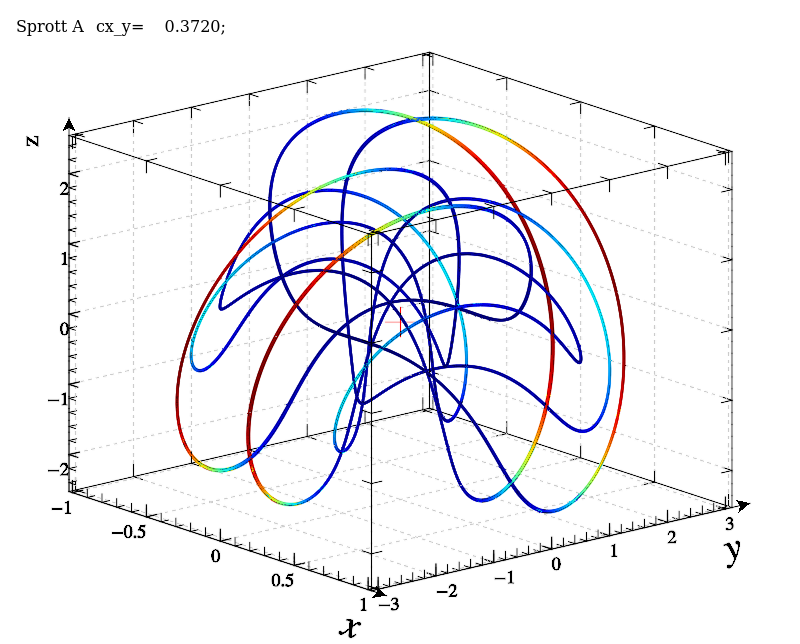
\includegraphics[width=0.49\textwidth]{p/cha/spr_a/sprott_a-p_xyz_cx_y=0x372.png}
  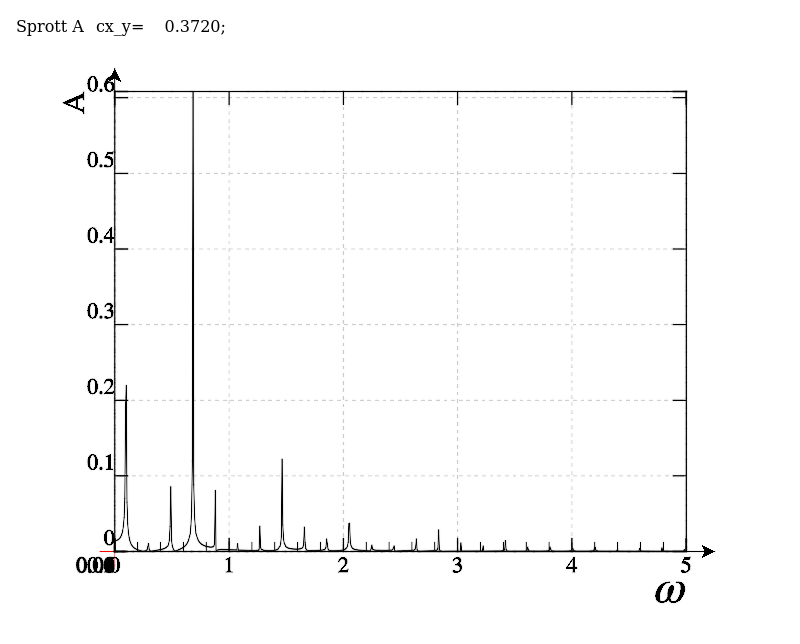
\includegraphics[width=0.49\textwidth]{p/cha/spr_a/sprott_a_f-p_f_cx_y=0x372.png}
}
\caption{Аттрактор и спектр системы (\ref{atu:eq:spr_a}) при $ c_{x_y} =0.372 $.
  Сложно-периодический режим.
}
\label{atu:f:spr_a_p_0372}
\end{figure}

При этом, в диапазоне $c_{x_y} \in [0.1 ; 0.7] $
наблюдаются перестройки структуры аттрактора, а при относительно больших
значениях данного параметра аттрактор представляет собой полый тор.

\begin{figure}[htb!]
\centerline{
  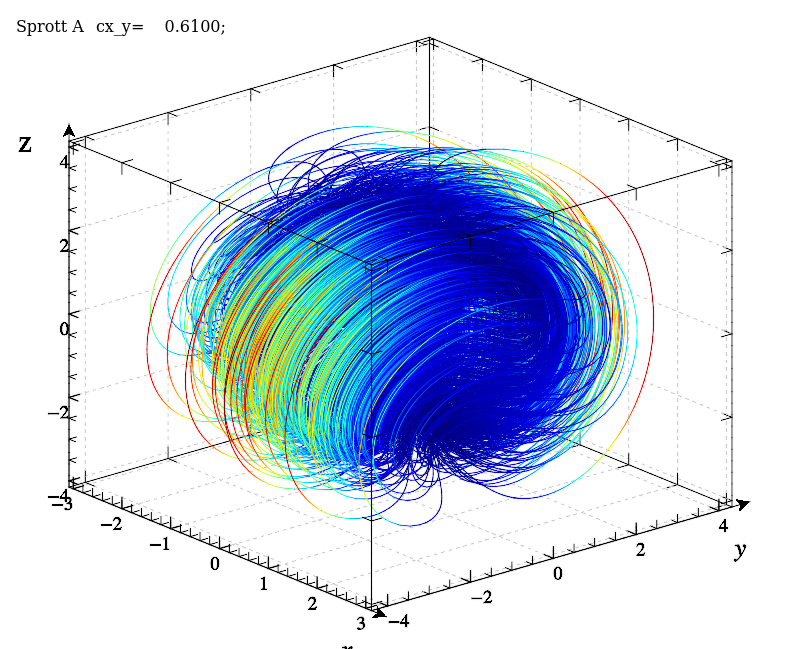
\includegraphics[width=0.49\textwidth]{p/cha/spr_a/sprott_a-p_xyz_cx_y=0x610.png}
  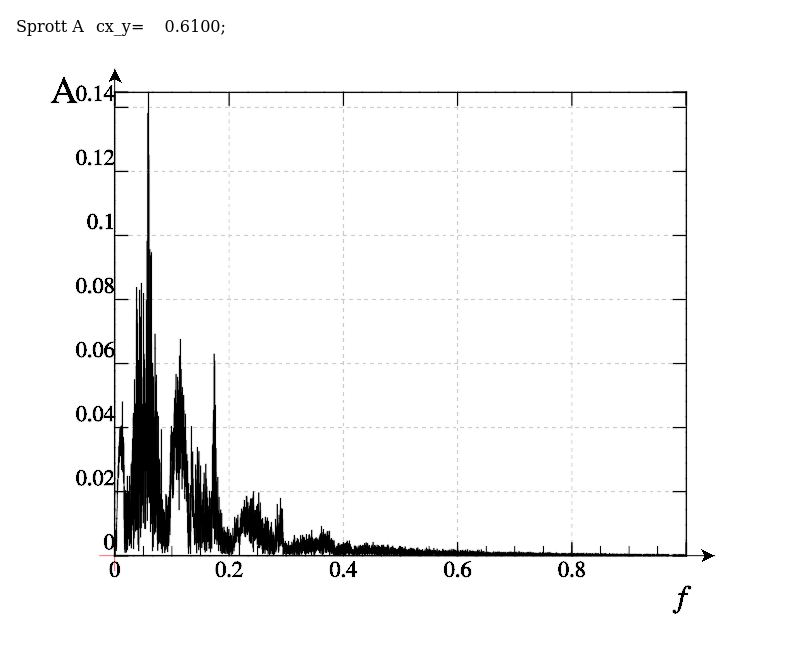
\includegraphics[width=0.49\textwidth]{p/cha/spr_a/sprott_a_f-p_f_cx_y=0x610.png}
}
\caption{Аттрактор и спектр системы (\ref{atu:eq:spr_a}) при $ c_{x_y} =0.610 $.
  Хаотический режим
}
\label{atu:f:spr_a_p_0610}
\end{figure}




Важной особенностью поведения этой системы является то, что при $ c_{x_y} \ge 1 $
в спектре системы имеются очень ограниченные участки сплошного спектра~(рис.~\ref{atu:f:spr_a_p_1000}).
При этом, как и для получения корректного спектра, так и для обнаружения ``разбегания'' траекторий
необходимо моделирование системы на протяжении достаточно длительного
(по сравнению с многими схожими системами) модельного времени.

\begin{figure}[htb!]
\centerline{
  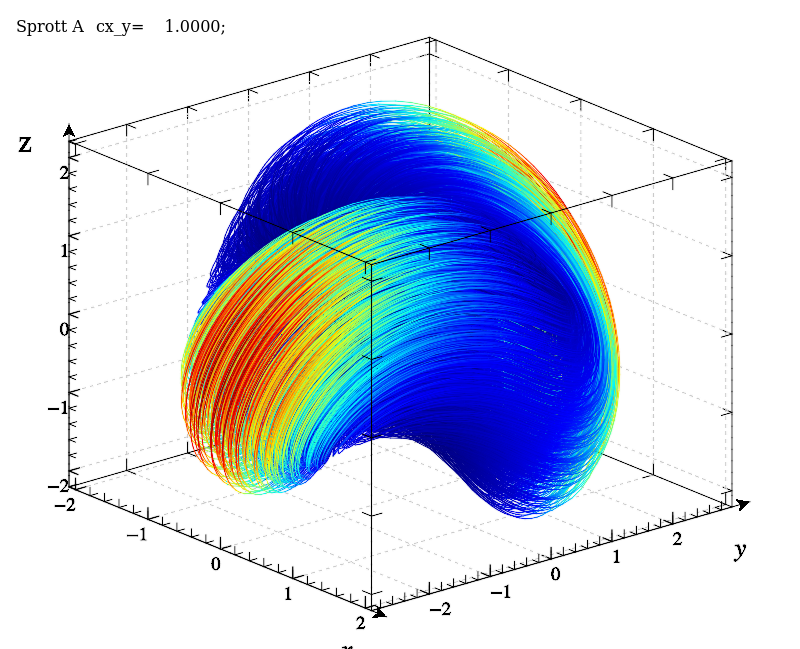
\includegraphics[width=0.49\textwidth]{p/cha/spr_a/sprott_a-p_xyz_cx_y=1x000.png}
  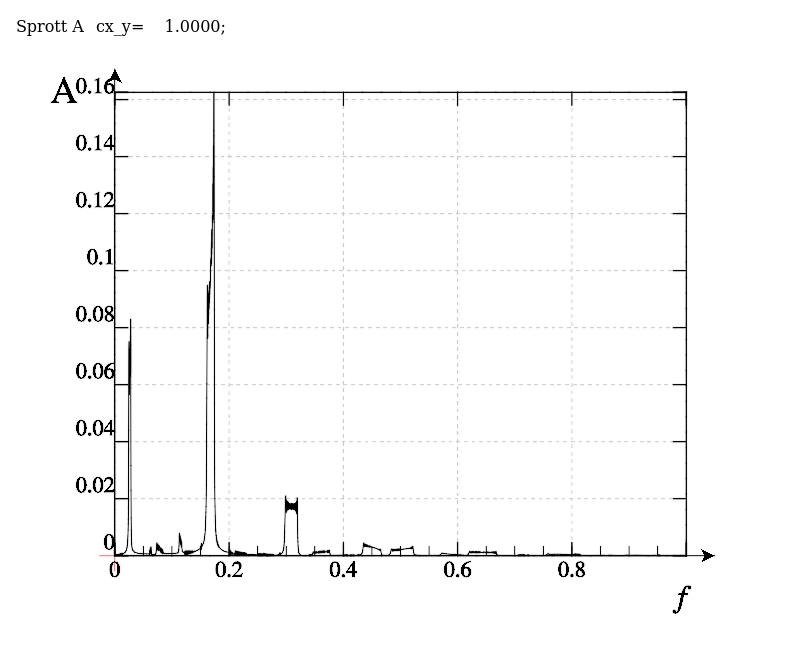
\includegraphics[width=0.49\textwidth]{p/cha/spr_a/sprott_a_f-p_f_cx_y=1x000.png}
}
\caption{Аттрактор и спектр системы (\ref{atu:eq:spr_a}) при $ c_{x_y} =1.0 $.
}
\label{atu:f:spr_a_p_1000}
\end{figure}


Рассмотрим зависимости $q_{*}(c_{x_y}) $ (рис.~\ref{atu:f:spr_a_q})
для системы (\ref{atu:eq:spr_a}). Анализ этих зависимостей
даёт практически однозначный ответ о возможном виде критерия -- $q_{x^2}$.
Второй кандидат -- $q_{x}$ обладает меньшей линейностью,
значения критериев, в которые не входит $x$, практически не зависят от $c_{c_y}$,
а вид критериев $q_{xy}$ и $q_{xz}$ ничем не лучше, чем у $q_{x}$.
Таким образом, систему идентификации будем строить, используя критерий  $q_{x^2}$.

\begin{figure}[htb!]
\centerline{
  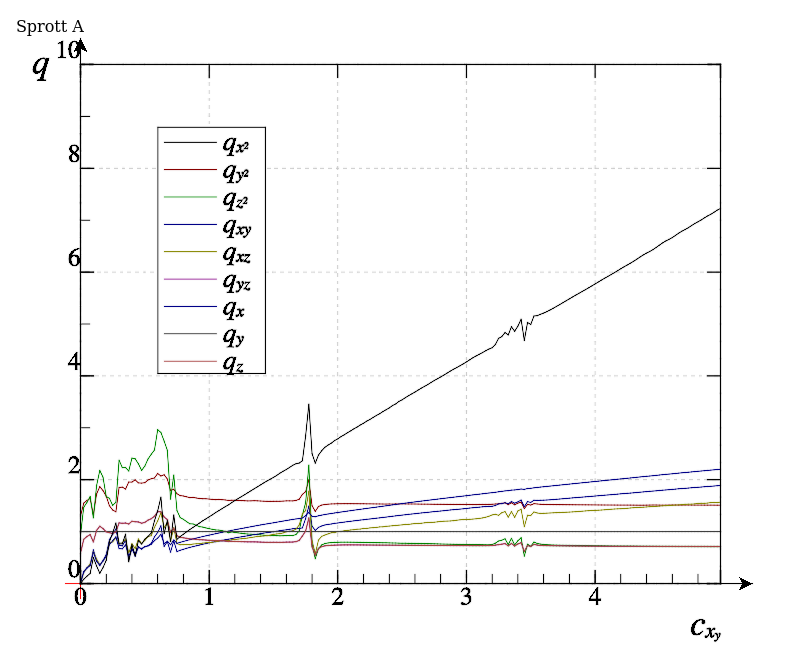
\includegraphics[width=0.60\textwidth]{p/cha/spr_a/sprott_a_q-p_c_x_y.png}
}
\caption{Зависимости $q_{*}(c_{x_y})$ для системы (\ref{atu:eq:spr_a}) }
\label{atu:f:spr_a_q}
\end{figure}

Нельзя не отметить, что в начальной области
$q_{x^2}(c_{x_y}) $, а именно там, где происходят постоянные
перестройки структуры аттрактора, ни один из рассматриваемых критериев
не имеет достаточной монотонности, что не даёт гарантии
построения работоспособной системы идентификации.
Для работы в этой области, скорее всего, требуется синтез специальных критериев.
Также, в окрестности точки $c_{x_y}=1.775$ аттрактор также резко изменяет свою структуру.
Так как это достаточно узкая окрестность,
то можно предположить, что мультиагентная система идентификации
не окажется неработоспособной в этой области, просто вырастет
ошибка идентификации.

Для проведения идентификации было выбрано два семейства методов:
qAuv5x3r.$q_{x^2}$ и
FAlv5.3r.$q_{x^2}$.

В соответствии с полученными данными, и используя
предложения~(\ref{atu:eq:po_t_sign}) и~(\ref{atu:eq:po_t_sin}),
определим тестовую задачу следующим образом:
\[
  c_{x_y}(t) \equiv p_o(t) \in (0, 5],
\]
%
\begin{equation}
  p_o(t) = p_0 +  U_{p} \sign \sin( \omega_{p} t ),
  \label{atu:eq:spr_a_po_t_sign}
\end{equation}
%
%
\begin{equation}
  p_o(t) = p_0 +  U_{p} \sin( \omega_{p} t ),
  \label{atu:eq:spr_a_po_t_sin}
\end{equation}
%
где:
$p_0 = 2.8$, $U_p=1.9$, $\omega_p=0.04$.

На рис.~\ref{atu:f:spr_a_id_qAuv5.3r.q_x2_sign} представлены результаты
методом qAuv5.3r.$q_{x^2}$. Аналогично системе Лоренца, на левом графике представлена
динамика перемещения каждой из подвижных моделей,
а на правом -- 4 способа определения $p_{id}(t)$:
$p_{ge}$, $p_{le}$, $p_{ee}$ и $p_{xe}$.
В первую очередь, следует отметить различие между процессами
идентификации этим методом данной системы и система Лоренца.
Зависимость $p_{xe}(t)$, в данном случае демонстрирует
высокий уровень колебаний, и следовательно,
худшие результаты поиска. При этом,
остальные подходы к определению $p_{id}$
демонстрируют схожие между собой результаты.
$\overline{e}_{bm}=1.41$
$\overline{e}_{ba}=1.49$.


\begin{figure}[h!]
  \centerline{
    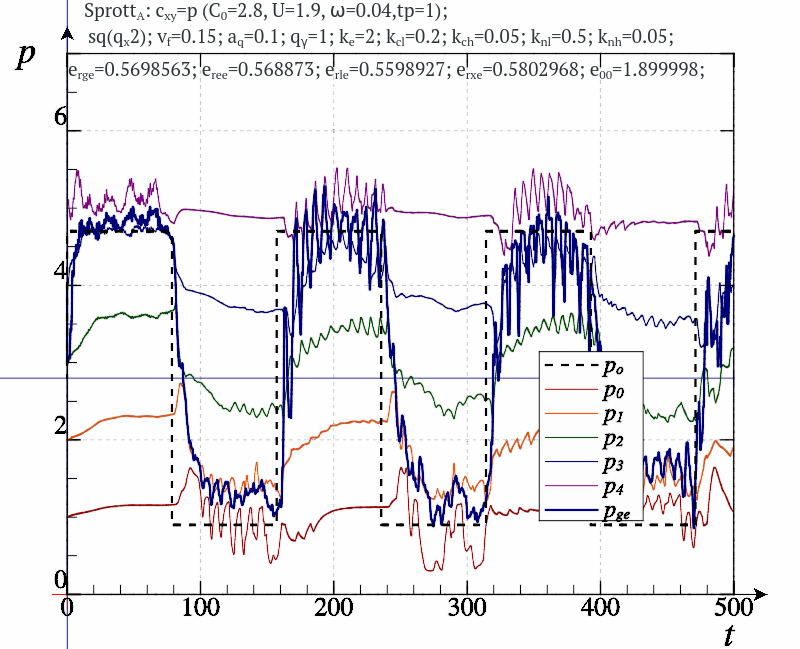
\includegraphics[width=0.49\textwidth]{p/cha/spr_a/qAuv5.3r/sprott_a_qAuv5_3r_qx2-p_t_pi_sign.png}
    \hfill
    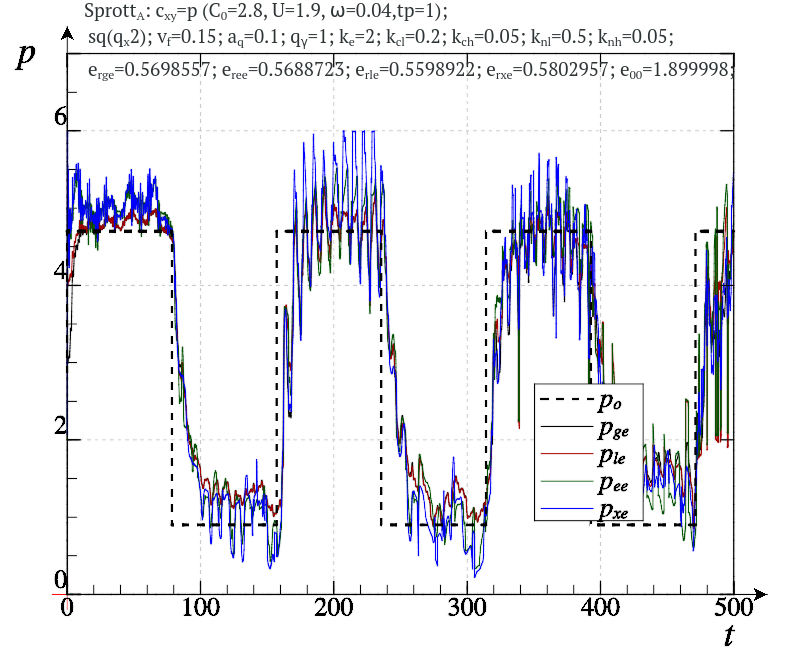
\includegraphics[width=0.49\textwidth]{p/cha/spr_a/qAuv5.3r/sprott_a_qAuv5_3r_qx2-p_t_pz_sign.png}
  }
  \caption{Процесс идентификации параметра ``$c_{x_y}$'' системы Sprott A методом qAuv5.3r.$q_{x^2}$ при условии~(\ref{atu:eq:spr_a_po_t_sign})}
  \label{atu:f:spr_a_id_qAuv5.3r.q_x2_sign}
\end{figure}

На рис.~\ref{atu:f:spr_a_id_qAuv5.3r.q_x2_sin} представлены аналогичные результаты,
но при условии плавного изменение значения $p_o(t)$. Также очевидно, что
как абсолютные, так и относительные значения ошибок идентификации в данном случае заметно
меньше, при сохранении общей картины.
$\overline{e}_{bm}=0.91$
и
$\overline{e}_{ba}=0.84$.

\begin{figure}[h!]
  \centerline{
    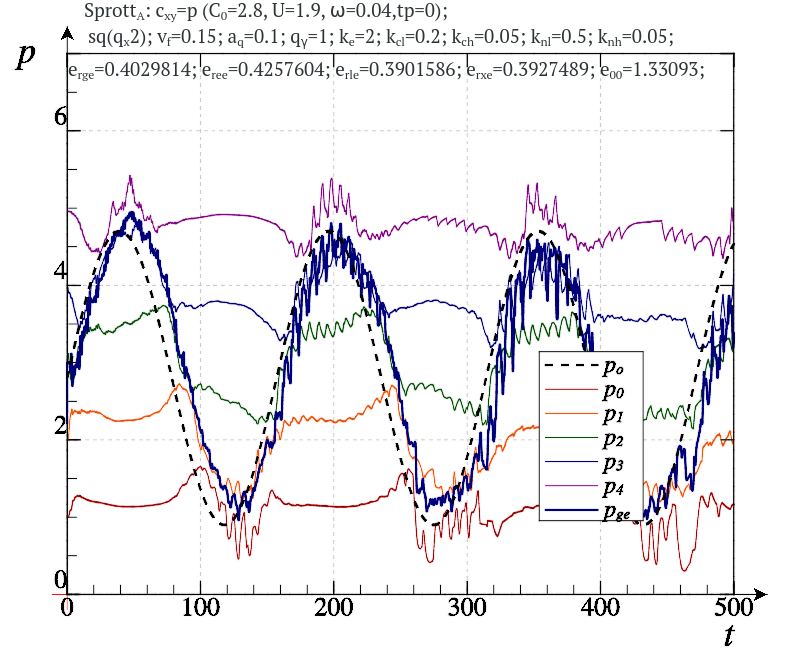
\includegraphics[width=0.49\textwidth]{p/cha/spr_a/qAuv5.3r/sprott_a_qAuv5_3r_qx2-p_t_pi_sin.png}
    \hfill
    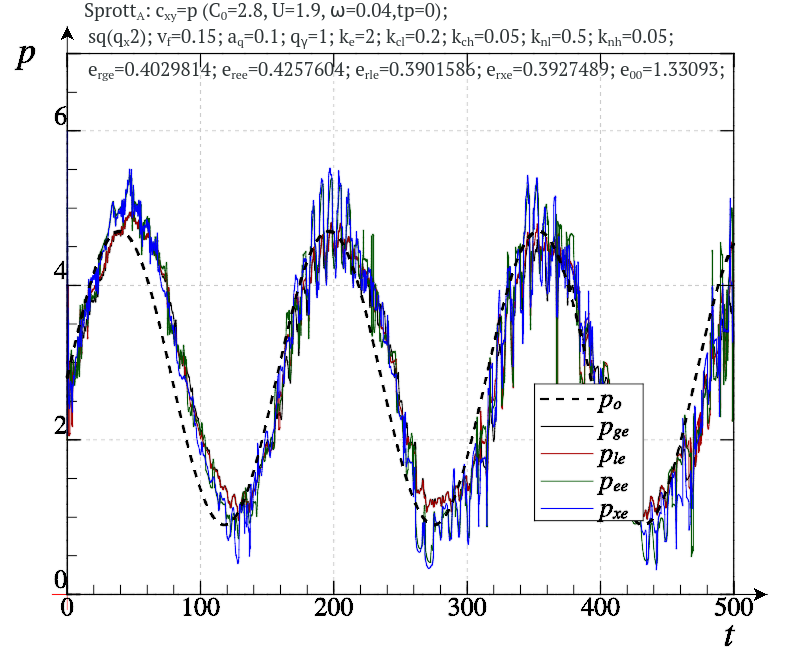
\includegraphics[width=0.49\textwidth]{p/cha/spr_a/qAuv5.3r/sprott_a_qAuv5_3r_qx2-p_t_pz_sin.png}
  }
  \caption{Процесс идентификации параметра ``$c_{x_y}$'' системы Sprott A методом qAuv5.3r.$q_{x^2}$ при условии~(\ref{atu:eq:spr_a_po_t_sin})}
  \label{atu:f:spr_a_id_qAuv5.3r.q_x2_sin}
\end{figure}


На рис.~\ref{atu:f:spr_a_id_FAlv5.3r.q_x2_sign} представлены результаты
методом FAlv5.3r.$q_{x^2}$.
$\overline{e}_{bm}=1.71$


\begin{figure}[h!]
  \centerline{
    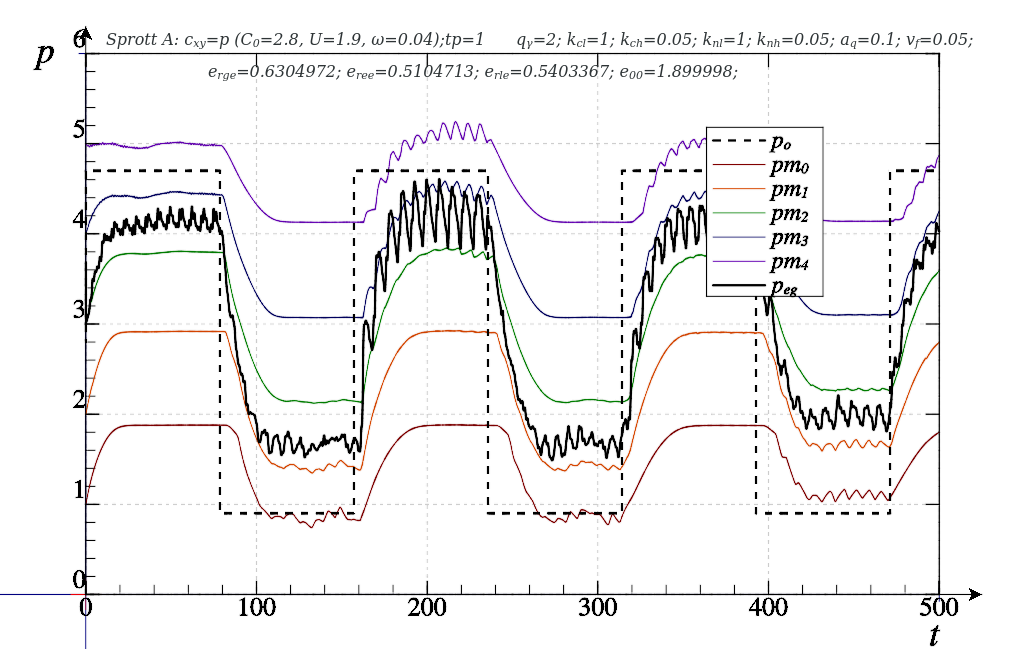
\includegraphics[width=0.49\textwidth]{p/cha/spr_a/FAlv5.3A/sprott_a_FAlv5x3r-pl_n_sign.png}
    \hfill
    \includegraphics[width=0.49\textwidth]{p/cha/spr_a/FAlv5.3A/sprott_a_FAlv5x3r-p_p_sign.png}
  }
  \caption{Процесс идентификации параметра ``$c_{x_y}$'' системы Sprott A методом FAlv5.3r.$q_{x^2}$ при условии~(\ref{atu:eq:spr_a_po_t_sign})}
  \label{atu:f:spr_a_id_FAlv5.3r.q_x2_sign}
\end{figure}

На рис.~\ref{atu:f:spr_a_id_FAlv5.3r.q_x2_sin} представлены аналогичные результаты,
но при условии плавного изменение значения параметра объекта. Очевидно, что
как абсолютные, так и относительные значения ошибок идентификации в данном случае заметно
меньше, при сохранении общей картины.
$\overline{e}_{bm}=0.87$

\begin{figure}[h!]
  \centerline{
    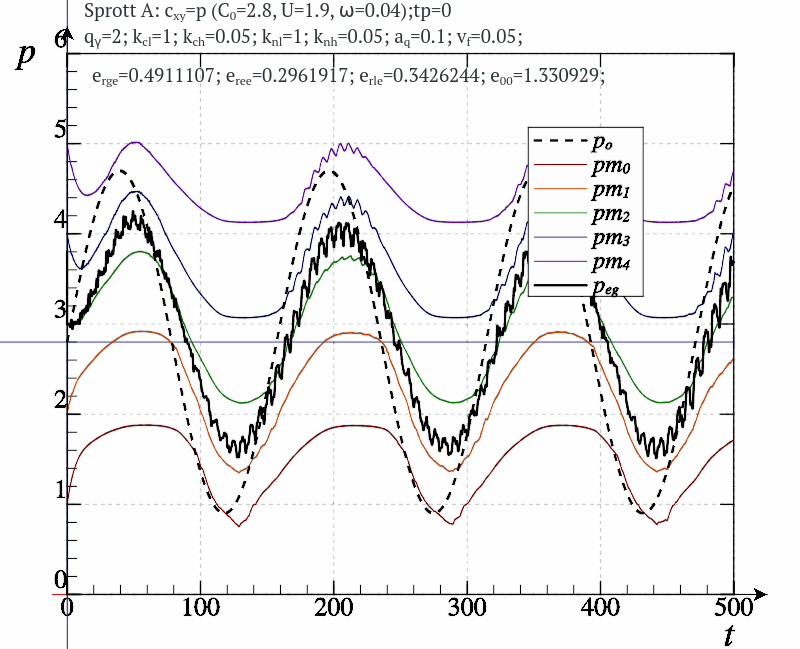
\includegraphics[width=0.49\textwidth]{p/cha/spr_a/FAlv5.3A/sprott_a_FAlv5x3r-pl_n_sin.png}
    \hfill
    \includegraphics[width=0.49\textwidth]{p/cha/spr_a/FAlv5.3A/sprott_a_FAlv5x3r-p_p_sin.png}
  }
  \caption{Процесс идентификации параметра ``$c_{x_y}$'' системы Sprott A методом FAlv5.3r.$q_{x^2}$ при условии~(\ref{atu:eq:spr_a_po_t_sin})}
  \label{atu:f:spr_a_id_FAlv5.3r.q_x2_sin}
\end{figure}




Рассмотрим влияние параметров системы идентификации на
ошибки идентификации.

Первый параметр --
$a_q$, определяющий характерное время усреднения критерия.

На рис.~\ref{atu:f:spr_a_a_q_qAuv5.3r.q_x2} представлены зависимости
$\overline{e}_{r*}(a_q)$ при применении метода qAuv5.3r.$q_{x^2}$.

\begin{figure}[h!]
  \centerline{
    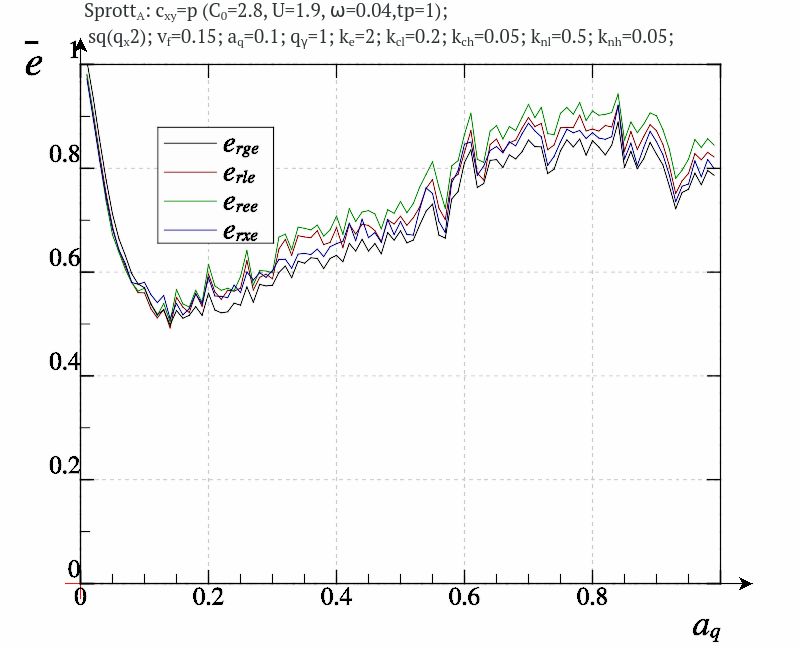
\includegraphics[width=0.49\textwidth]{p/cha/spr_a/qAuv5.3r/sprott_a_qAuv5_3r_qx2-p_a_q_e_sign.png}
    \hfill
    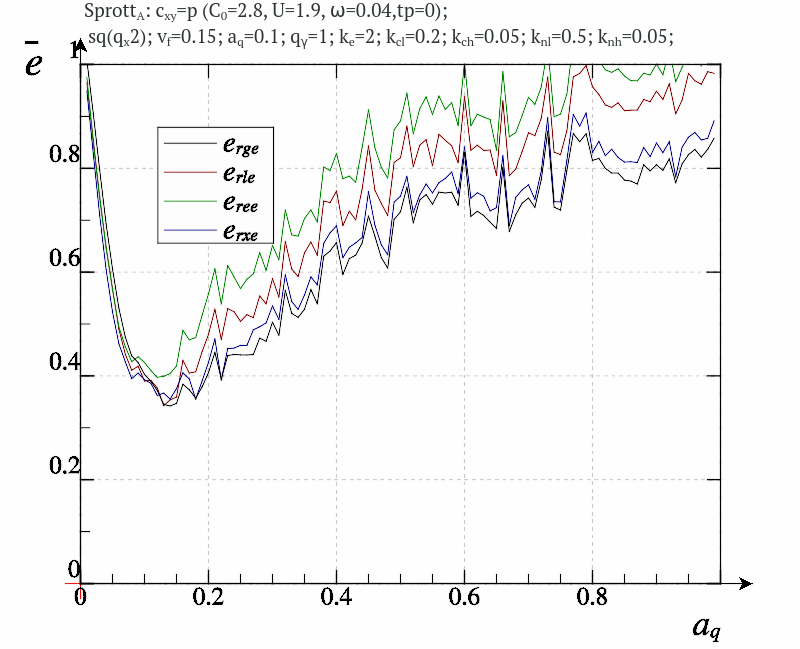
\includegraphics[width=0.49\textwidth]{p/cha/spr_a/qAuv5.3r/sprott_a_qAuv5_3r_qx2-p_a_q_e_sin.png}
  }
  \caption{Зависимости $\overline{e}_{r*}(a_q)$ при идентификации системы Sprott A методом qAuv5.3r.$q_{x^2}$
   при~(\ref{atu:eq:spr_a_po_t_sign}) и (\ref{atu:eq:spr_a_po_t_sin})}
  \label{atu:f:spr_a_a_q_qAuv5.3r.q_x2}
\end{figure}


На рис.~\ref{atu:f:spr_a_a_q_FAlv5.3r.q_x2} представлены зависимости
$\overline{e}_{r*}(a_q)$ при применении метода FAlv5.3r.$q_{x^2}$.

\begin{figure}[h!]
  \centerline{
    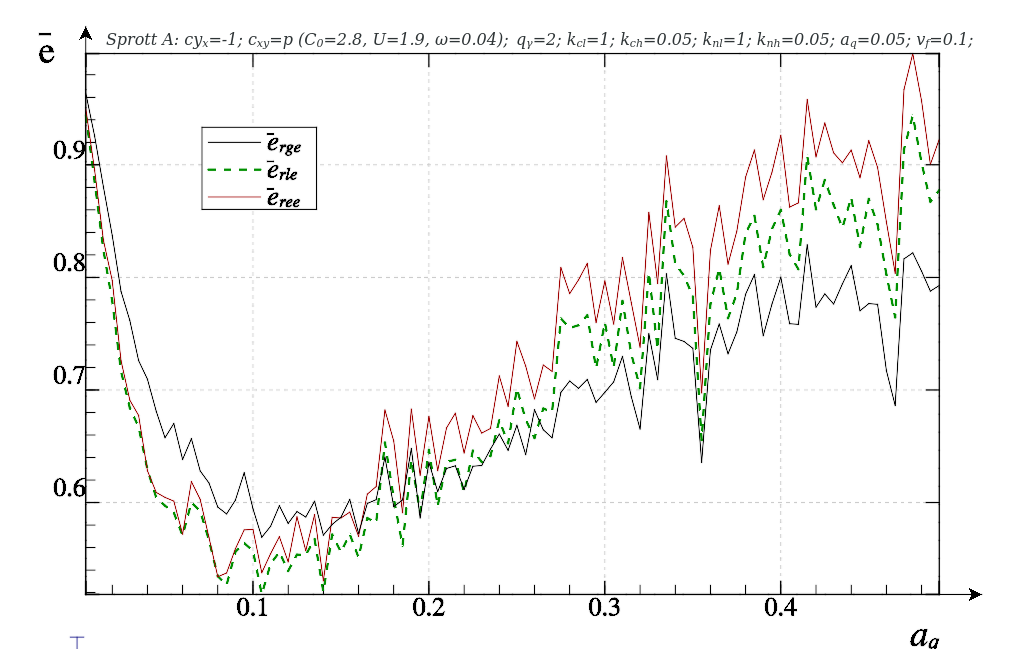
\includegraphics[width=0.49\textwidth]{p/cha/spr_a/FAlv5.3A/sprott_a_FAlv5x3r-p_a_q_e_sign.png}
    \hfill
    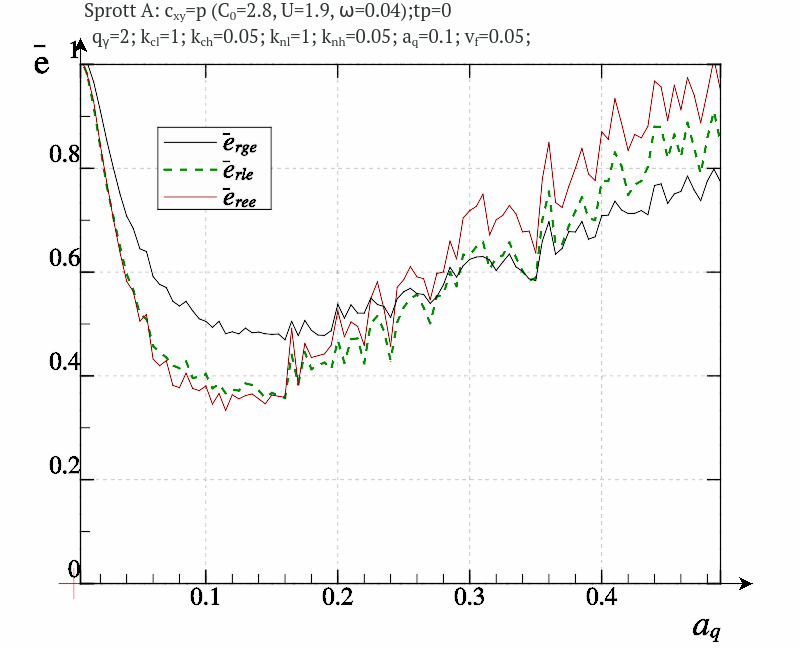
\includegraphics[width=0.49\textwidth]{p/cha/spr_a/FAlv5.3A/sprott_a_FAlv5x3r-p_a_q_e_sin.png}
  }
  \caption{Зависимости $\overline{e}_{r*}(a_q)$ при идентификации системы Sprott A методом FAlv5.3r.$q_{x^2}$
   при~(\ref{atu:eq:spr_a_po_t_sign}) и (\ref{atu:eq:spr_a_po_t_sin})}
  \label{atu:f:spr_a_a_q_FAlv5.3r.q_x2}
\end{figure}

Следующий параметр -- $q_\gamma$ должен больше влиять на процессы идентификации,
использующие для оценки $p_e$ функцию качества.

На рис.~\ref{atu:f:spr_a_qg_qAuv5.3r.q_x2} представлены зависимости
$\overline{e}_{r*}(q_\gamma)$ при применении метода qAuv5.3r.$q_{x^2}$.

\begin{figure}[h!]
  \centerline{
    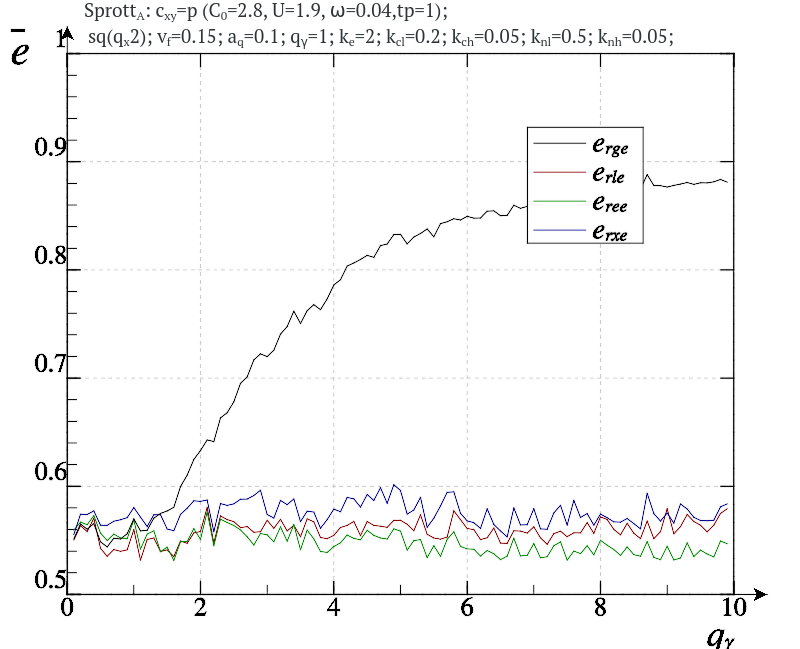
\includegraphics[width=0.49\textwidth]{p/cha/spr_a/qAuv5.3r/sprott_a_qAuv5_3r_qx2-p_qgamma_e_sign.png}
    \hfill
    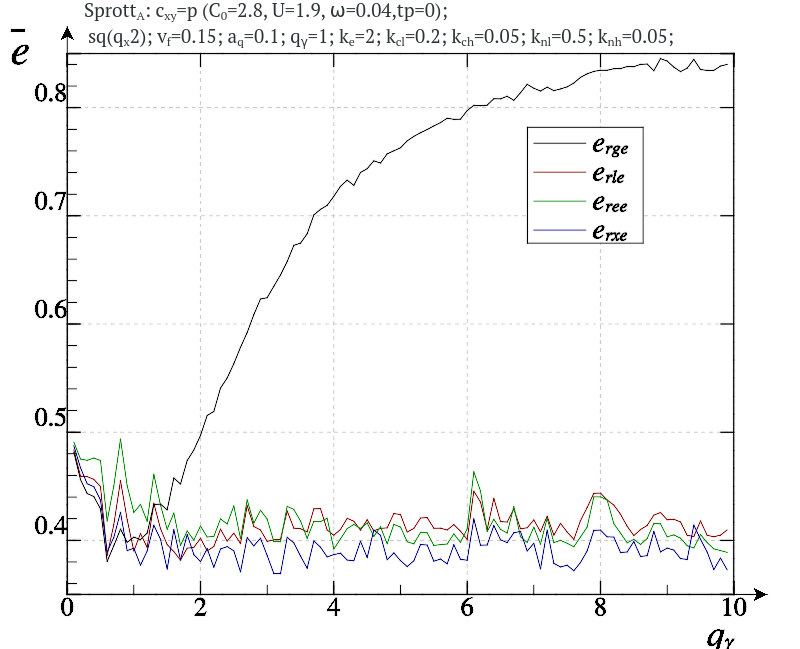
\includegraphics[width=0.49\textwidth]{p/cha/spr_a/qAuv5.3r/sprott_a_qAuv5_3r_qx2-p_qgamma_e_sin.png}
  }
  \caption{Зависимости $\overline{e}_{r*}(q_\gamma)$ при идентификации системы Sprott A методом qAuv5.3r.$q_{x^2}$
   при~(\ref{atu:eq:spr_a_po_t_sign}) и (\ref{atu:eq:spr_a_po_t_sin})}
  \label{atu:f:spr_a_qg_qAuv5.3r.q_x2}
\end{figure}

На рис.~\ref{atu:f:spr_a_qg_FAlv5.3r.q_x2} представлены зависимости
$\overline{e}_{r*}(q_\gamma)$ при применении метода FAlv5.3r.$q_{x^2}$.

\begin{figure}[h!]
  \centerline{
    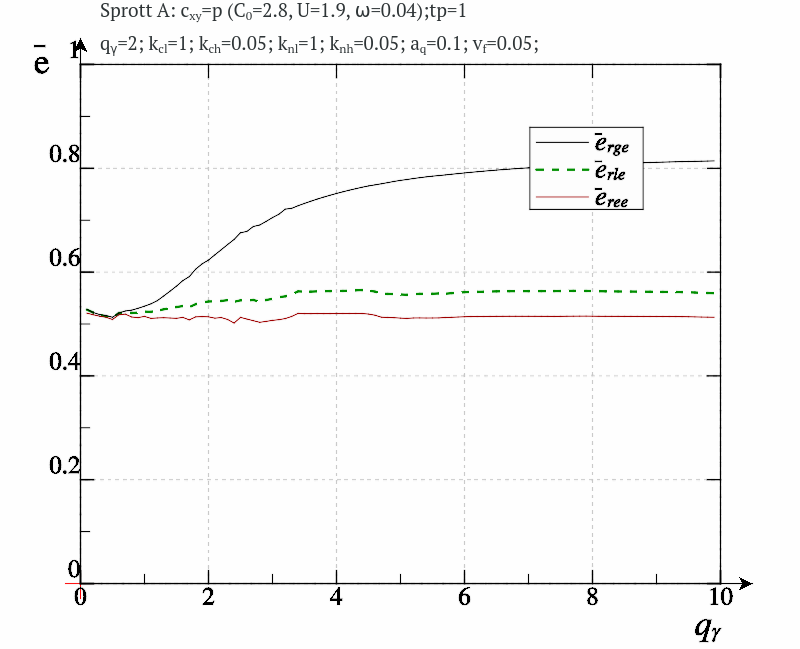
\includegraphics[width=0.49\textwidth]{p/cha/spr_a/FAlv5.3A/sprott_a_FAlv5x3r-p_qg_e_sign.png}
    \hfill
    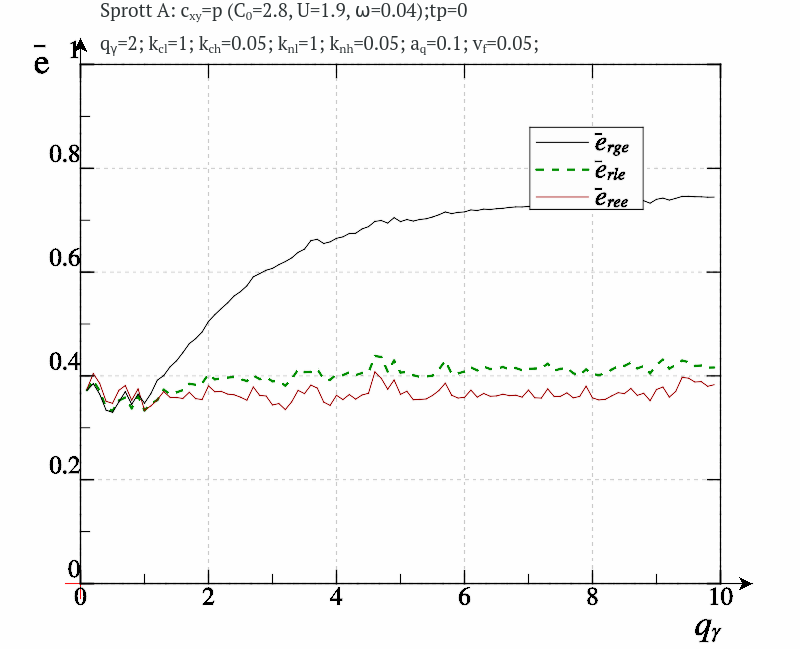
\includegraphics[width=0.49\textwidth]{p/cha/spr_a/FAlv5.3A/sprott_a_FAlv5x3r-p_qg_e_sin.png}
  }
  \caption{Зависимости $\overline{e}_{r*}(q_\gamma)$ при идентификации системы Sprott A методом FAlv5.3r.$q_{x^2}$
   при~(\ref{atu:eq:spr_a_po_t_sign}) и (\ref{atu:eq:spr_a_po_t_sin})}
  \label{atu:f:spr_a_qg_FAlv5.3r.q_x2}
\end{figure}

Зависимость $\overline{e}( q_\gamma )$ % (рис.~\ref{atu:f:spr_a_e_qgamma})
свидетельствует о довольно слабом влиянии этого параметра
на динамику системы идентификации.
Проявляются робастные свойства поисковых агентов.



Параметр $v_f$, определяющий динамику поисковых агентов:


На рис.~\ref{atu:f:spr_a_v_f_qAuv5.3r.q_x2} представлены зависимости
$\overline{e}_{r*}(v_f)$ при применении метода qAuv5.3r.$q_{x^2}$.

\begin{figure}[h!]
  \centerline{
    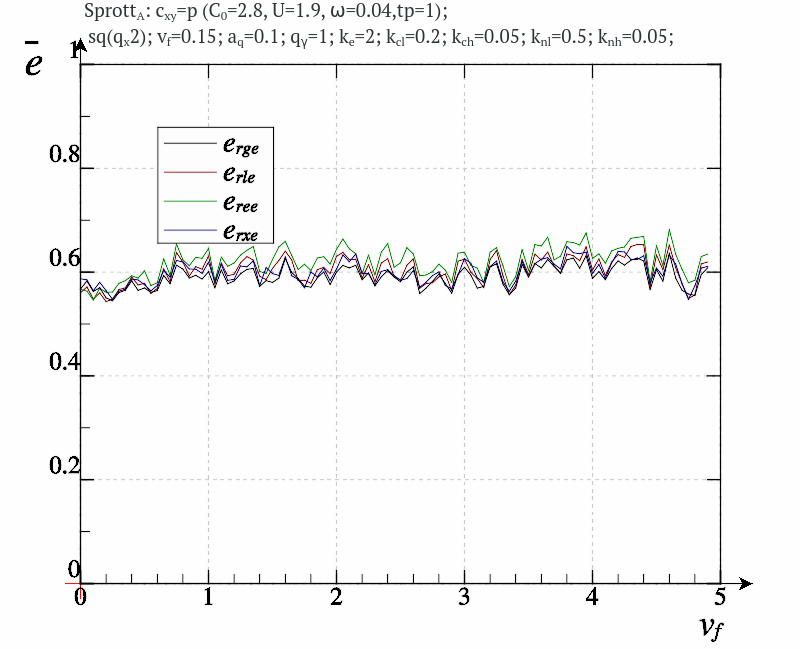
\includegraphics[width=0.49\textwidth]{p/cha/spr_a/qAuv5.3r/sprott_a_qAuv5_3r_qx2-p_v_f_e_sign.png}
    \hfill
    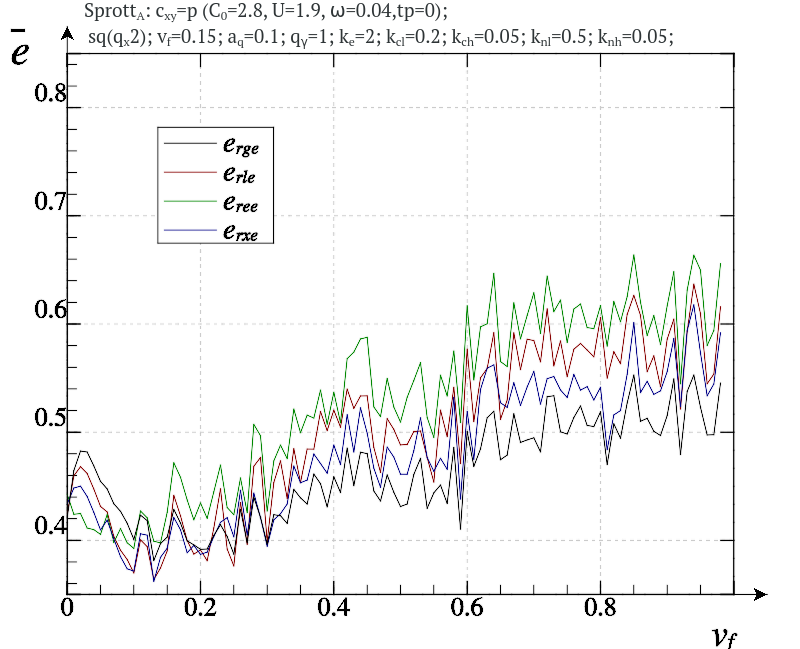
\includegraphics[width=0.49\textwidth]{p/cha/spr_a/qAuv5.3r/sprott_a_qAuv5_3r_qx2-p_v_f_e_sin.png}
  }
  \caption{Зависимости $\overline{e}_{r*}(v_f)$ при идентификации системы Sprott A методом qAuv5.3r.$q_{x^2}$
   при~(\ref{atu:eq:spr_a_po_t_sign}) и (\ref{atu:eq:spr_a_po_t_sin})}
  \label{atu:f:spr_a_v_f_qAuv5.3r.q_x2}
\end{figure}

На рис.~\ref{atu:f:spr_a_v_f_FAlv5.3r.q_x2} представлены зависимости
$\overline{e}_{r*}(v_f)$ при применении метода FAlv5.3r.$q_{x^2}$.

\begin{figure}[h!]
  \centerline{
    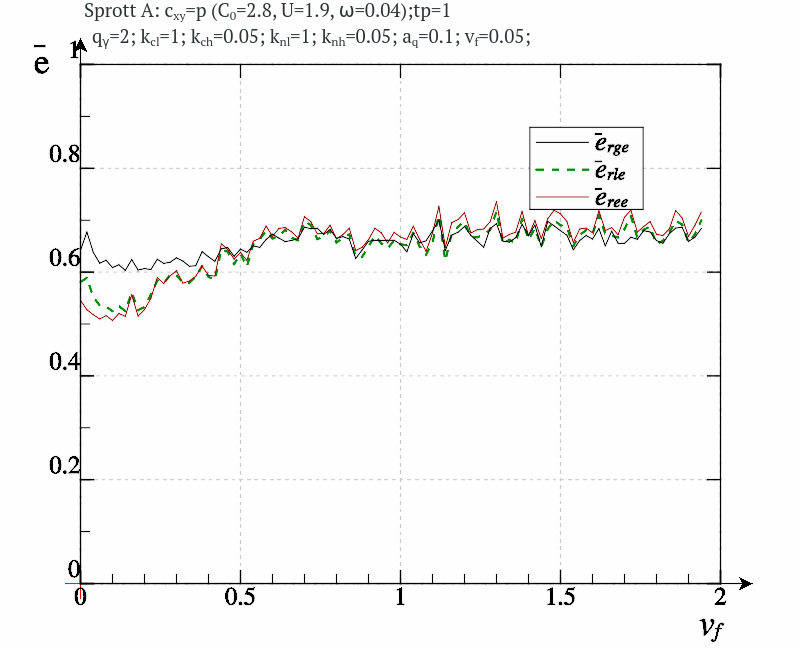
\includegraphics[width=0.49\textwidth]{p/cha/spr_a/FAlv5.3A/sprott_a_FAlv5x3r-p_v_f_e_sign.png}
    \hfill
    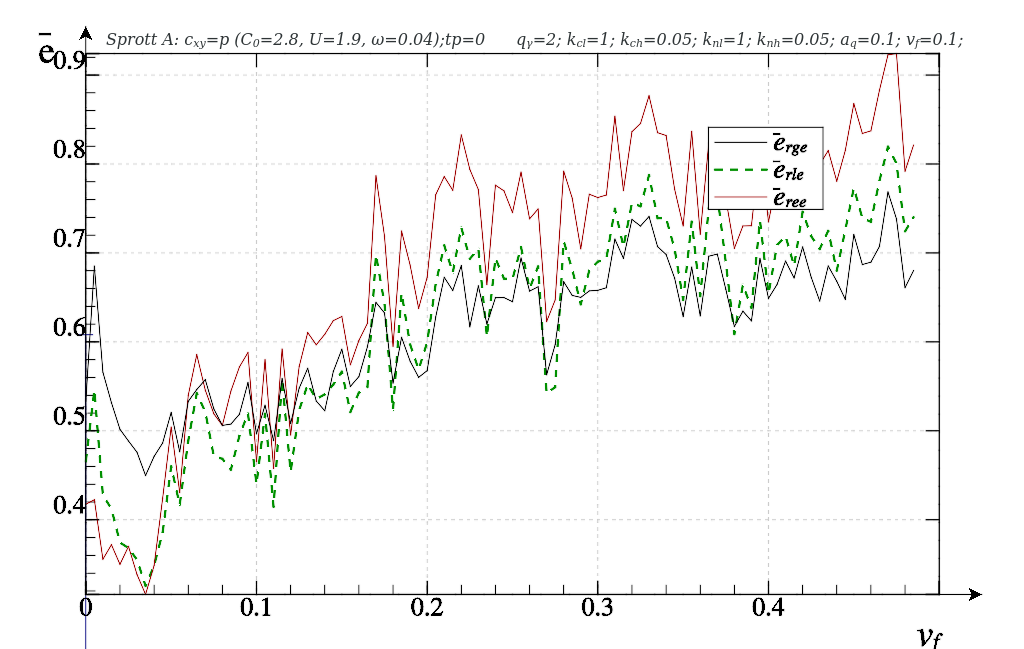
\includegraphics[width=0.49\textwidth]{p/cha/spr_a/FAlv5.3A/sprott_a_FAlv5x3r-p_v_f_e_sin.png}
  }
  \caption{Зависимости $\overline{e}_{r*}(v_f)$ при идентификации системы Sprott A методом FAlv5.3r.$q_{x^2}$
   при~(\ref{atu:eq:spr_a_po_t_sign}) и (\ref{atu:eq:spr_a_po_t_sin})}
  \label{atu:f:spr_a_v_f_FAlv5.3r.q_x2}
\end{figure}

Параметр $k_e$, определяющий соотношение сил, действующих
на поисковый агент:


На рис.~\ref{atu:f:spr_a_k_e_qAuv5.3r.q_x2} представлены зависимости
$\overline{e}_{r*}(k_e)$ при применении метода qAuv5.3r.$q_{x^2}$.

\begin{figure}[h!]
  \centerline{
    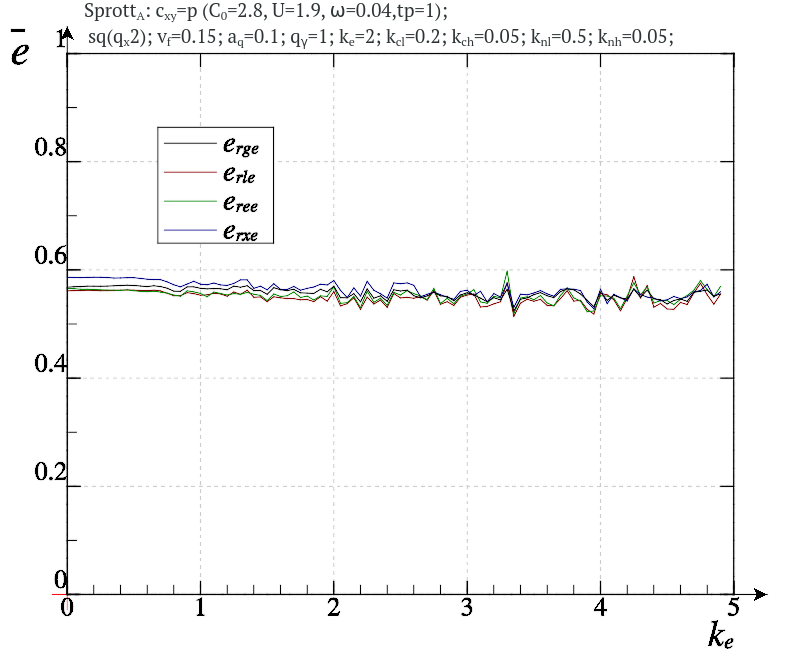
\includegraphics[width=0.49\textwidth]{p/cha/spr_a/qAuv5.3r/sprott_a_qAuv5_3r_qx2-p_k_e_e_sign.png}
    \hfill
    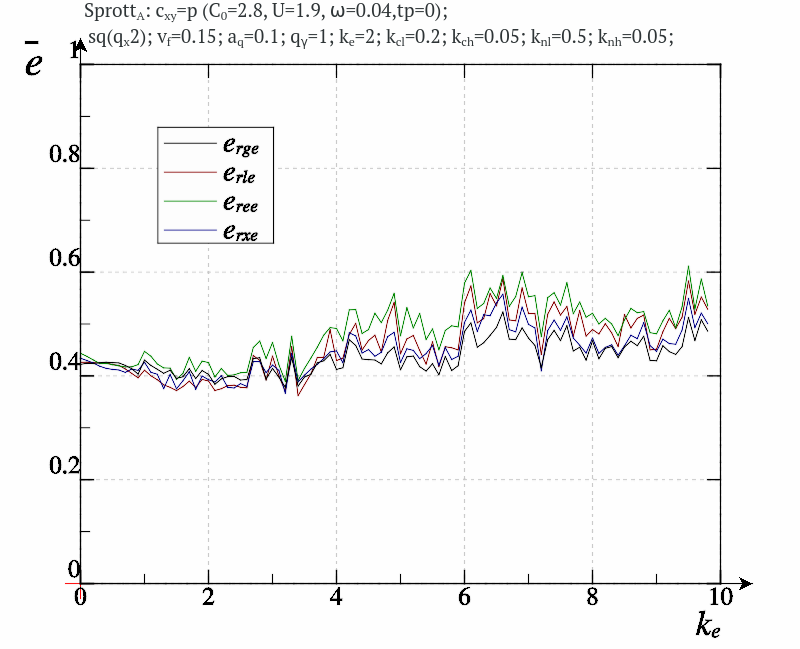
\includegraphics[width=0.49\textwidth]{p/cha/spr_a/qAuv5.3r/sprott_a_qAuv5_3r_qx2-p_k_e_e_sin.png}
  }
  \caption{Зависимости $\overline{e}_{r*}(k_e)$ при идентификации системы Sprott A методом qAuv5.3r.$q_{x^2}$
   при~(\ref{atu:eq:spr_a_po_t_sign}) и (\ref{atu:eq:spr_a_po_t_sin})}
  \label{atu:f:spr_a_k_e_qAuv5.3r.q_x2}
\end{figure}

На рис.~\ref{atu:f:spr_a_k_e_FAlv5.3r.q_x2} представлены зависимости
$\overline{e}_{r*}(k_e)$ при применении метода FAlv5.3r.$q_{x^2}$.

\begin{figure}[h!]
  \centerline{
    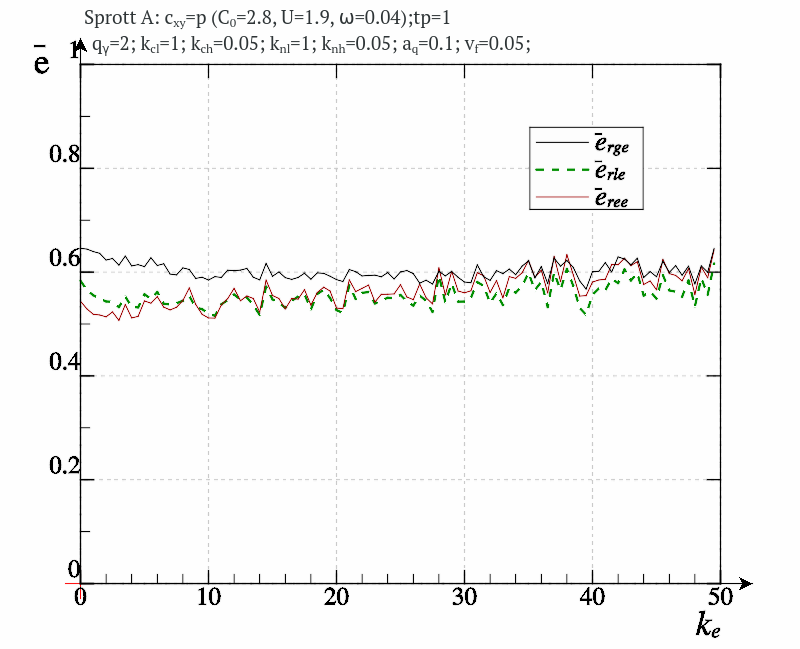
\includegraphics[width=0.49\textwidth]{p/cha/spr_a/FAlv5.3A/sprott_a_FAlv5x3r-p_ke_e_sign.png}
    \hfill
    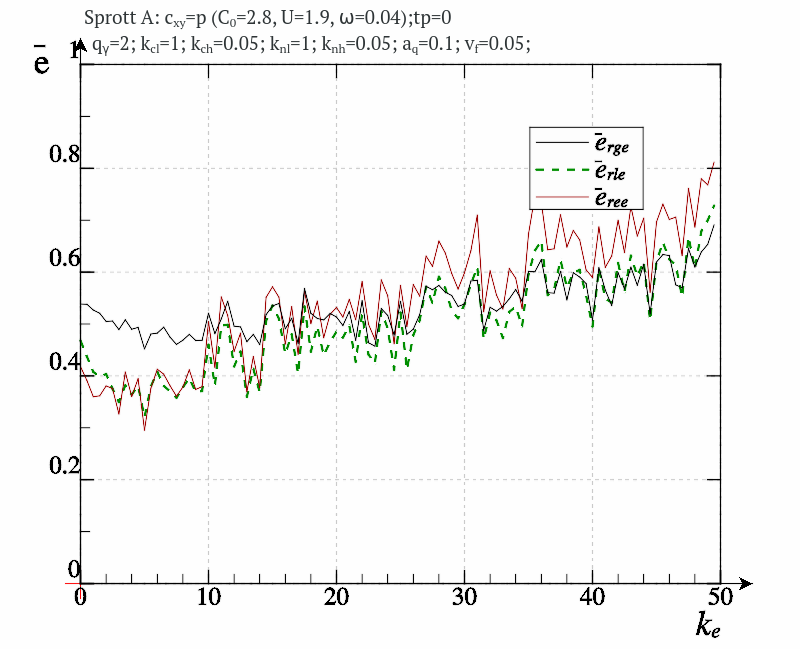
\includegraphics[width=0.49\textwidth]{p/cha/spr_a/FAlv5.3A/sprott_a_FAlv5x3r-p_ke_e_sin.png}
  }
  \caption{Зависимости $\overline{e}_{r*}(k_e)$ при идентификации системы Sprott A методом FAlv5.3r.$q_{x^2}$
   при~(\ref{atu:eq:spr_a_po_t_sign}) и (\ref{atu:eq:spr_a_po_t_sin})}
  \label{atu:f:spr_a_k_e_FAlv5.3r.q_x2}
\end{figure}




Таким образом, для хаотической системы ``Sprott A''
удалось создать и критерий идентификации и работоспособную систему идентификации
на основании энергетического критерия вида $q_{x^2}$.


